% Copyright 2004 by Till Tantau <tantau@users.sourceforge.net>.
%
% In principle, this file can be redistributed and/or modified under
% the terms of the GNU Public License, version 2.
%
% However, this file is supposed to be a template to be modified
% for your own needs. For this reason, if you use this file as a
% template and not specifically distribute it as part of a another
% package/program, I grant the extra permission to freely copy and
% modify this file as you see fit and even to delete this copyright
% notice.

\documentclass{beamer}

% There are many different themes available for Beamer. A comprehensive
% list with examples is given here:
% http://deic.uab.es/~iblanes/beamer_gallery/index_by_theme.html
% You can uncomment the themes below if you would like to use a different
% one:
%\usetheme{AnnArbor}
%\usetheme{Antibes}
%\usetheme{Bergen}
%\usetheme{Berkeley}
%\usetheme{Berlin}
%\usetheme{Boadilla}
%\usetheme{boxes}
%\usetheme{CambridgeUS}
%\usetheme{Copenhagen}
%\usetheme{Darmstadt}
%\usetheme{default}
%\usetheme{Frankfurt}
%\usetheme{Goettingen}
%\usetheme{Hannover}
%\usetheme{Ilmenau}
%\usetheme{JuanLesPins}
%\usetheme{Luebeck}
\usetheme{Madrid}
%\usetheme{Malmoe}
%\usetheme{Marburg}
%\usetheme{Montpellier}
%\usetheme{PaloAlto}
%\usetheme{Pittsburgh}
%\usetheme{Rochester}
%\usetheme{Singapore}
%\usetheme{Szeged}
%\usetheme{Warsaw}

\title{Gate Problems on Control Systems}

% A subtitle is optional and this may be deleted
\subtitle{EC 2016 Q46}

\author{Piyush Kumar Uttam}
% - Give the names in the same order as the appear in the paper.
% - Use the \inst{?} command only if the authors have different
%   affiliation.

\institute[Indian Institute of Technology,Hyderabad] % (optional, but mostly needed)
{
  \inst{1}%
  Department of Electrical Engineering\\
  Indian Institute of Technology,Hyderabad
 }
% - Use the \inst command only if there are several affiliations.
% - Keep it simple, no one is interested in your street address.

\date{}
% - Either use conference name or its abbreviation.
% - Not really informative to the audience, more for people (including
%   yourself) who are reading the slides online

\subject{Theoretical Computer Science}
% This is only inserted into the PDF information catalog. Can be left
% out.

% If you have a file called "university-logo-filename.xxx", where xxx
% is a graphic format that can be processed by latex or pdflatex,
% resp., then you can add a logo as follows:

% \pgfdeclareimage[height=0.5cm]{university-logo}{university-logo-filename}
% \logo{\pgfuseimage{university-logo}}

% Delete this, if you do not want the table of contents to pop up at
% the beginning of each subsection:
\AtBeginSubsection[]
{
  \begin{frame}<beamer>{Outline}
    \tableofcontents[currentsection,currentsubsection]
  \end{frame}
}




\begin{document}


\begin{frame}
\titlepage
\end{frame}



\begin{frame}{Question}
\begin{block}

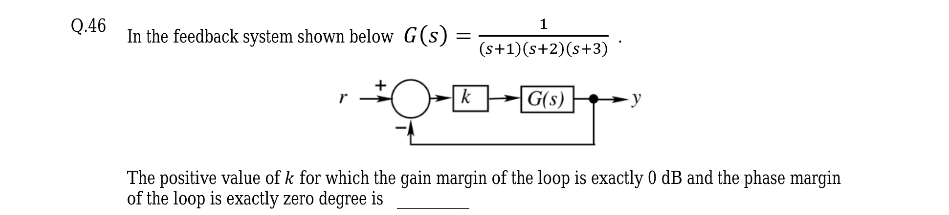
\includegraphics[scale=0.4]{1.png}

\end{block}
\end{frame}
%\begin{frame}
%\tableofcontents
%\end{frame}

\begin{frame}{Theory}

\begin{block}

The gain margin is defined as the change in open-loop gain required to make the closed-loop system unstable. Systems with greater gain margins can withstand greater changes in system parameters before becoming unstable in closed-loop. 

\end{block} \vspace{16pt}
\begin{block}

The phase margin is defined as the change in open-loop phase shift required to make the closed-loop system unstable. The phase margin also measures the system's tolerance to time delay
\end{block} \vspace{16pt}




\end{frame}



\begin{frame}{Technique Description}
\begin{block}

As given in question we see that gain margin is 0 dB and phase margin is 0 degrees. This implies that system is just enough stable and will become destabilized on just small increase in gain. Hence the system is marginbally stable.
\end{block}

\begin{block}

The stability of the system can be checked by Routh-Hurwitz Stability Criterion 
\end{block}

\end{frame}


\begin{frame}{Routh-Hurwitz Stability Criterion}
\begin{block}

Necessary condition for Routh-Hurwitz Stability Criterion: The necessary condition is that the coefficients of the characteristic polynomial should be positive. This implies that all the roots of the characteristic equation should have negative real parts.

Sufficient condition for Routh-Hurwitz Stability Criterion:The sufficient condition is that all the elements of the first column of the Routh array should have the same sign. This means that all the elements of the first column of the Routh array should be either positive or negative.\vspace{16pt}
\includegraphics[scale=0.3]{pic2}
\end{block}

\end{frame}

\begin{frame}
The Routh array for characteristic equation $a_0s^n+a_1s^(n-1)+a_2s^(n-2)+a_3s^(n-3).....+a_n$
\begin{table}[]
\begin{tabular}{lllll}
$s^n$ & $a_0$ & $a_2$ &  &  \\
$s^(n-1)$ & $a_1$ & $a_3$ &  &  \\
$s^(n-2)$ & 2 & 0 &  &  \\
$s^(n-3)$ & 0 & 0 &  & 
\end{tabular}
\end{table}
\end{frame}

\begin{frame}{Solution}
The Routh array for equation $s^3+6s^2+11s^1+(6+k)$
\begin{table}[]
\begin{tabular}{lllll}
$s^3$ & 1            & 11    &  &  \\
$s^2$ & 6            & (6+k) &  &  \\
$s^1$ & $\frac{66-(6+K)}{6}$& 0     &  &  \\
$s^0$ & $(6+k)$        & 0     &  & 


\end{tabular}
\end{table}
Now since the system is marginally stable therefore $s^1$ row is $\geq$ 0\newline
Hence $\frac{66-(6+K)}{6}$$\geq$0
Hence k=60
\end{frame}
\begin{frame}{Verification using Plots}
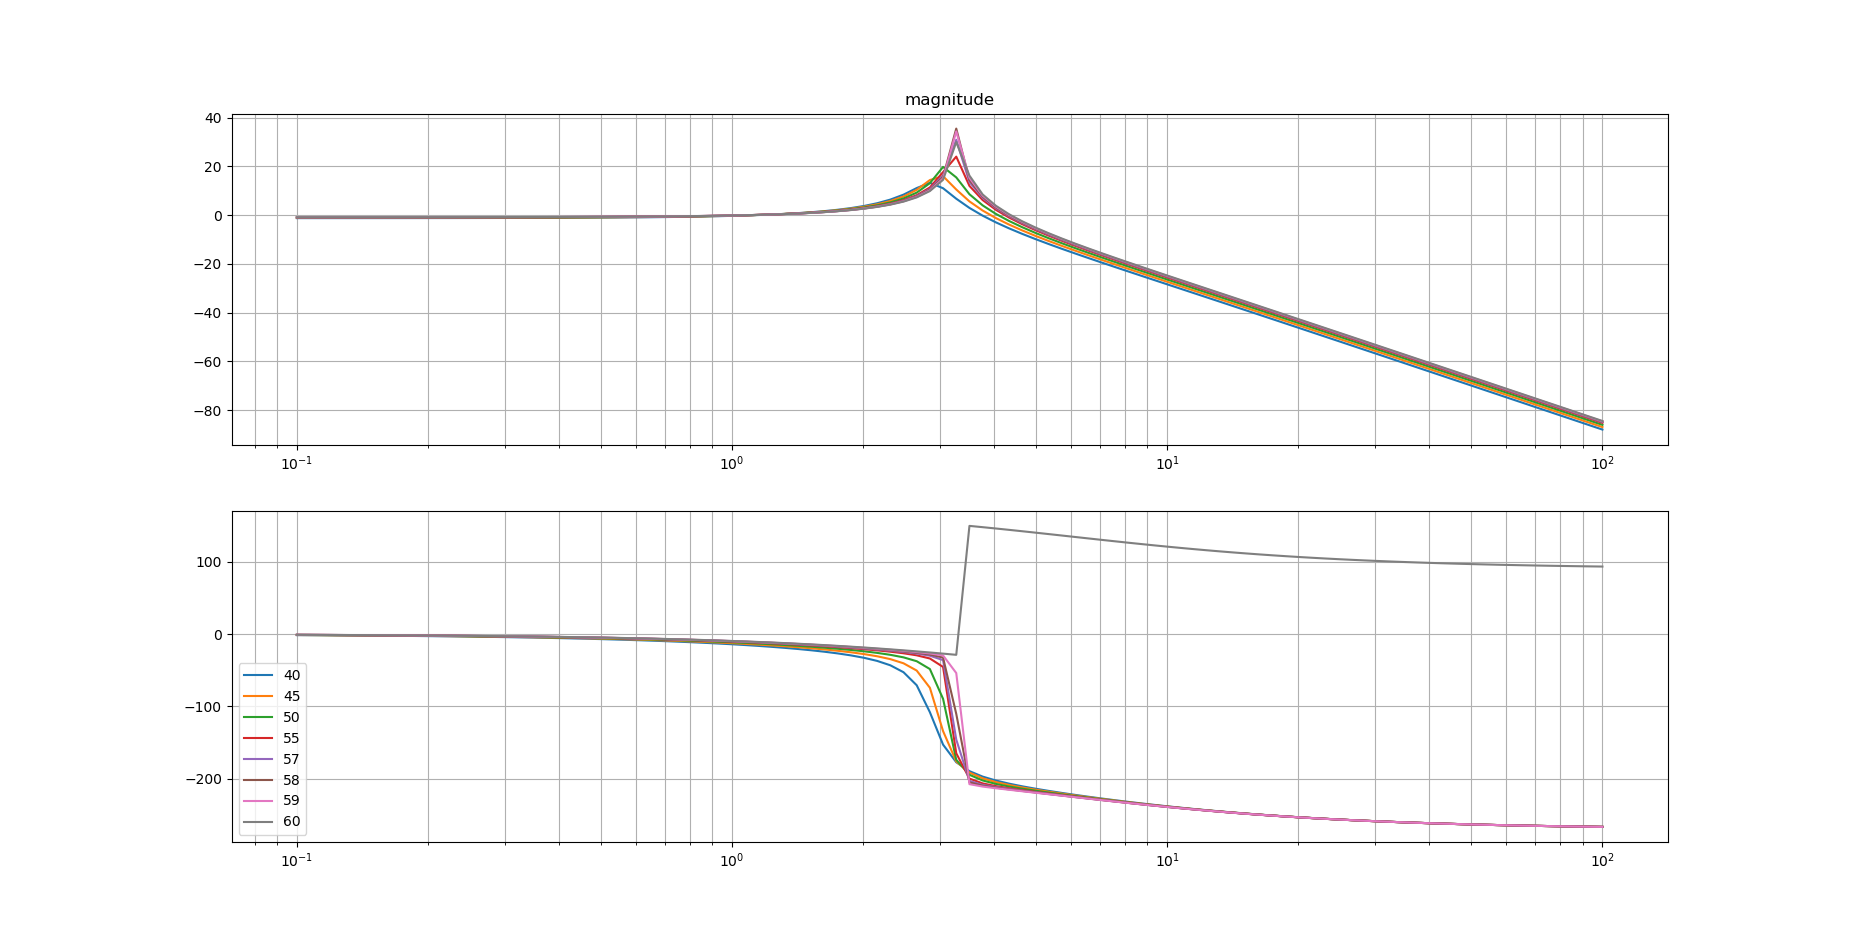
\includegraphics[scale=0.27]{bode2.png}

\end{frame}
\begin{frame}{Verification using Plots}
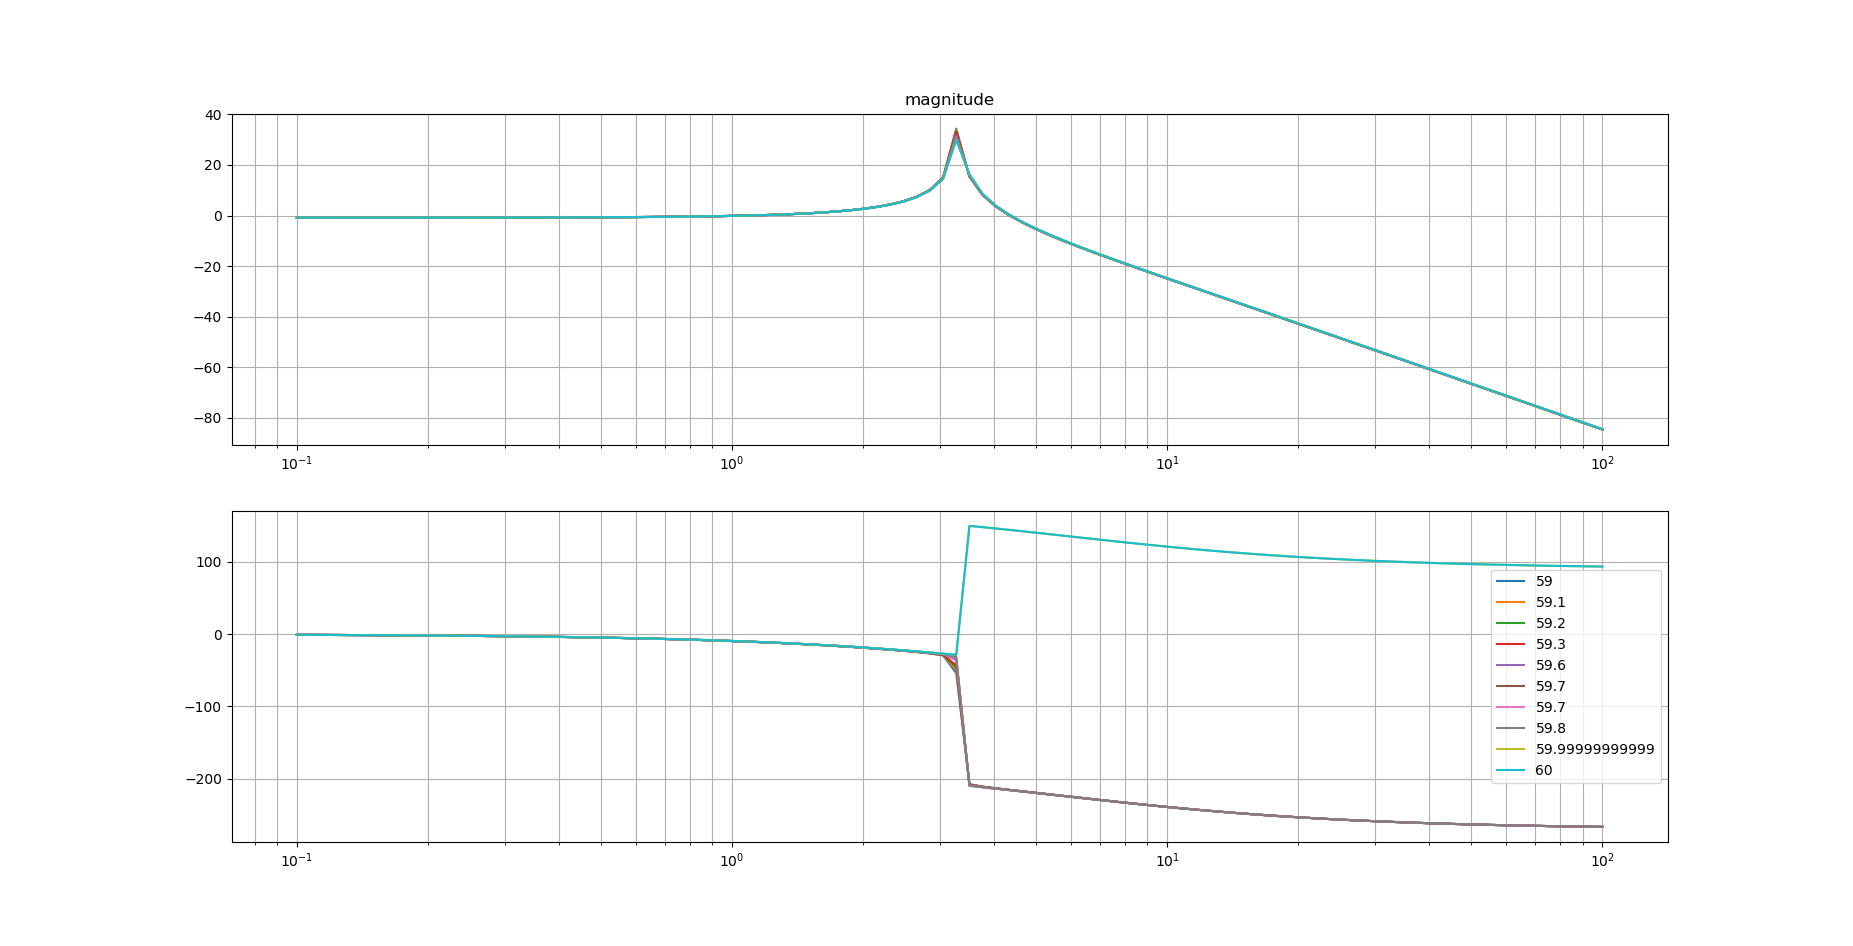
\includegraphics[scale=0.27]{bode.png}

\end{frame}
\end{document}
